\section{Data structure}

\subsection{Représentation}
{
\logo{}
\begin{frame}
\frametitle{Data structure}
\begin{figure}[h!]
    \begin{tikzpicture}
    \node[]{
        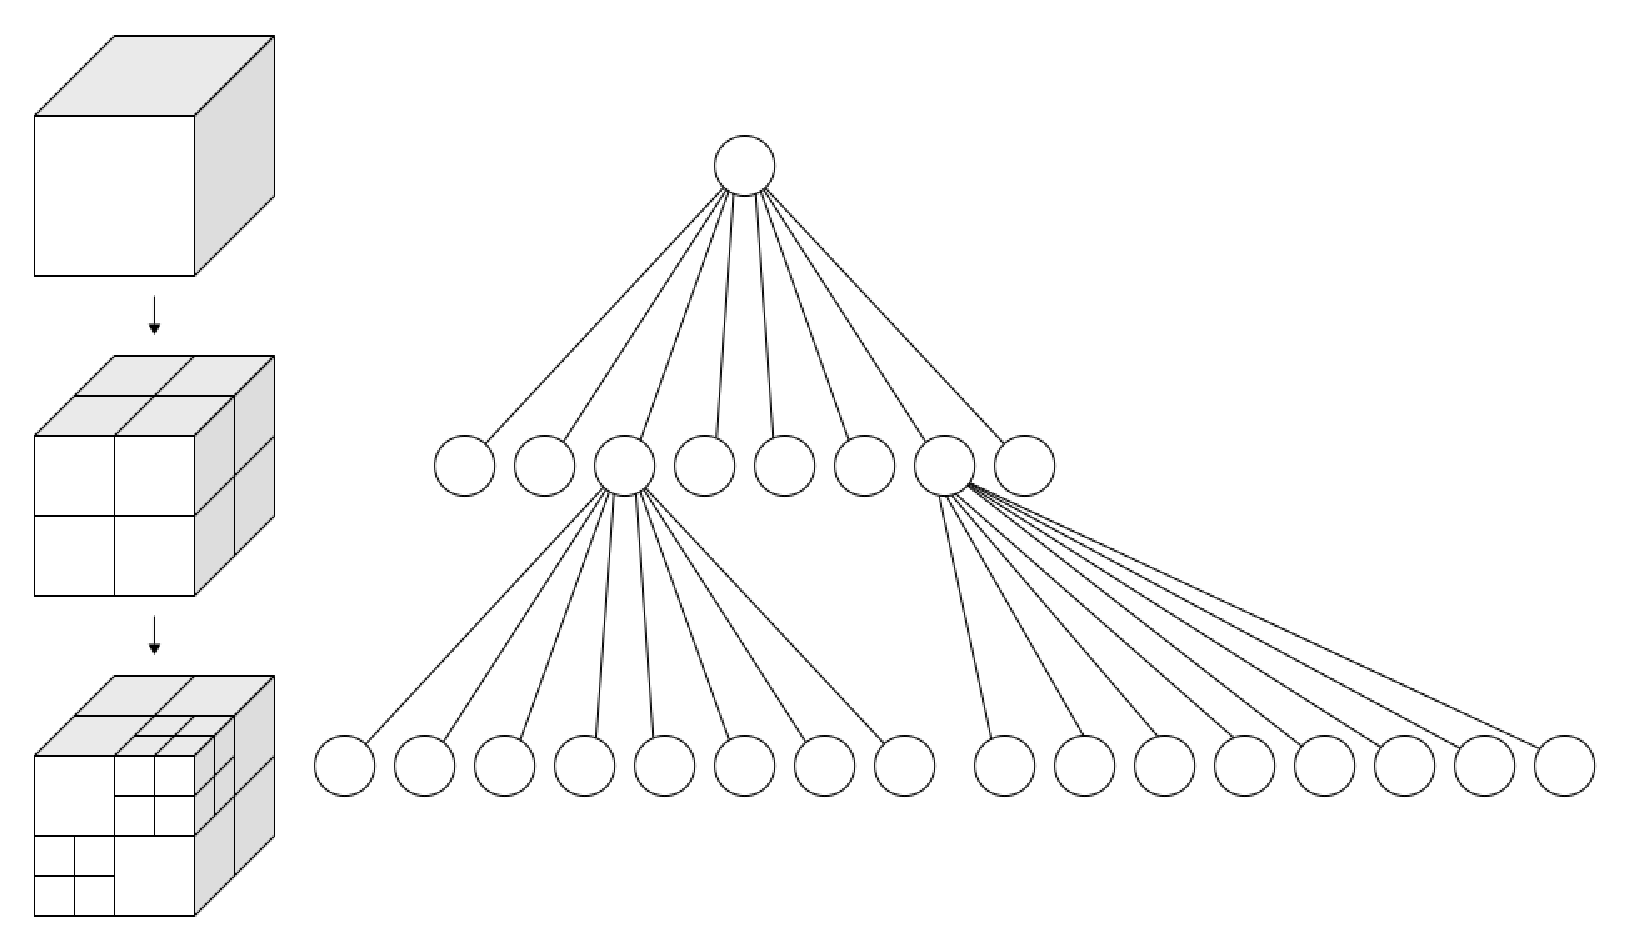
\includegraphics[width=0.8\textwidth]{octree}};
    \end{tikzpicture}
    \caption{Représentation d'un octree}
\end{figure}
\end{frame}
}

\subsection{Complexités}
\begin{frame}
\frametitle{Complexités}
\begin{itemize}
    \itemsep1.5em
    \item Accès : $O(M\frac{\log(N)}{\log(M)})$
    \item Temps de recherche de voisins jusqu'à 10 fois plus rapide pour < 1K
        atomes
    \item Parcours entier à l'arbre
    \item Utilisation de Queue pour le dessin
\end{itemize}
\end{frame}
